\documentclass[aspectratio=169,12pt]{beamer}
\usepackage[utf8]{inputenc}
\usepackage{amsmath, amssymb}
\usepackage{booktabs}
\usepackage{colortbl}
\usepackage{hyperref}
\usepackage{makecell}
\usepackage{ragged2e}
\usepackage{tikz}
\usetikzlibrary{arrows.meta, positioning, shapes.geometric, calc, tikzmark, shapes.misc, fit, decorations.pathreplacing, matrix}
\usepackage{tcolorbox}
\usepackage{array}
\usepackage{listings}
\usepackage{pgfkeys}
\usetheme{Madrid}

% Custom colors
\definecolor{correctgreen}{RGB}{0,150,0}
\definecolor{incorrectred}{RGB}{200,0,0}
\definecolor{counterblue}{RGB}{70,130,255}
\definecolor{highlightyellow}{RGB}{255,230,100}
\definecolor{lightblue}{RGB}{200,230,250}
\definecolor{darkblue}{RGB}{0,100,200}
\definecolor{lightgreen}{RGB}{144,238,144}

% Define asmcode command for assembly code formatting
\newcommand{\asmcode}[1]{\vspace{-0.2cm}\tiny\texttt{#1}}

\pgfkeys{
    /OOO/.is family, /OOO,
    default/.style = {
        % RAT registers
        R1 = {}, R2 = {}, R3 = {}, R4 = {}, R5 = {},
        R6 = {}, R7 = {}, R8 = {}, R9 = {}, R10 = {},
        % ROB cells (2 columns x 9 rows)
        rob11 = {}, rob12 = {},
        rob21 = {}, rob22 = {},
        rob31 = {}, rob32 = {},
        rob41 = {}, rob42 = {},
        rob51 = {}, rob52 = {},
        rob61 = {}, rob62 = {},
        rob71 = {}, rob72 = {},
        rob81 = {}, rob82 = {},
        rob91 = {}, rob92 = {},
        % ROB markers
        robmark1 = {rob1}, robmark2 = {rob2}, robmark3 = {rob3},
        robmark4 = {rob4}, robmark5 = {rob5}, robmark6 = {rob6},
        robmark7 = {rob7}, robmark8 = {rob8}, robmark9 = {rob9},
        % IDQ cells
        idq1 = {}, idq2 = {}, idq3 = {}, idq4 = {}, idq5 = {}, idq6 = {},
        % RS cells
        rs1 = {}, rs2 = {}, rs3 = {}, rs4 = {},
        % RS markers
        rsmark1 = {rs1}, rsmark2 = {rs2}, rsmark3 = {rs3}, rsmark4 = {rs4},
        % MOB cells
        mob1 = {}, mob2 = {},
        % MOB markers
        mobmark1 = {mob1}, mobmark2 = {mob2},
        % Execute cells
        exec1 = {}, exec2 = {},
        % Retire cells
        ret1 = {}, ret2 = {},
        % Retire markers
        retmark1 = {ret1}, retmark2 = {ret2},
        % Number of rows/cols (for iteration purposes)
        rob rows = 9,
        idq rows = 6,
        rs rows = 4,
        mob rows = 2,
        execute rows = 2,
        retire cols = 2
    },
    % RAT mappings
    R1/.estore in = \prfOne,
    R2/.estore in = \prfTwo,
    R3/.estore in = \prfThree,
    R4/.estore in = \prfFour,
    R5/.estore in = \prfFive,
    R6/.estore in = \prfSix,
    R7/.estore in = \prfSeven,
    R8/.estore in = \prfEight,
    R9/.estore in = \prfNine,
    R10/.estore in = \prfTen,
    % ROB cell contents
    rob11/.estore in = \robOneOne, rob12/.estore in = \robOneTwo,
    rob21/.estore in = \robTwoOne, rob22/.estore in = \robTwoTwo,
    rob31/.estore in = \robThreeOne, rob32/.estore in = \robThreeTwo,
    rob41/.estore in = \robFourOne, rob42/.estore in = \robFourTwo,
    rob51/.estore in = \robFiveOne, rob52/.estore in = \robFiveTwo,
    rob61/.estore in = \robSixOne, rob62/.estore in = \robSixTwo,
    rob71/.estore in = \robSevenOne, rob72/.estore in = \robSevenTwo,
    rob81/.estore in = \robEightOne, rob82/.estore in = \robEightTwo,
    rob91/.estore in = \robNineOne, rob92/.estore in = \robNineTwo,
    % ROB markers
    robmark1/.estore in = \robMarkOne,
    robmark2/.estore in = \robMarkTwo,
    robmark3/.estore in = \robMarkThree,
    robmark4/.estore in = \robMarkFour,
    robmark5/.estore in = \robMarkFive,
    robmark6/.estore in = \robMarkSix,
    robmark7/.estore in = \robMarkSeven,
    robmark8/.estore in = \robMarkEight,
    robmark9/.estore in = \robMarkNine,
    % IDQ cell contents
    idq1/.estore in = \idqOne,
    idq2/.estore in = \idqTwo,
    idq3/.estore in = \idqThree,
    idq4/.estore in = \idqFour,
    idq5/.estore in = \idqFive,
    idq6/.estore in = \idqSix,
    % RS cell contents
    rs1/.estore in = \rsOne,
    rs2/.estore in = \rsTwo,
    rs3/.estore in = \rsThree,
    rs4/.estore in = \rsFour,
    % RS markers
    rsmark1/.estore in = \rsMarkOne,
    rsmark2/.estore in = \rsMarkTwo,
    rsmark3/.estore in = \rsMarkThree,
    rsmark4/.estore in = \rsMarkFour,
    % MOB cell contents
    mob1/.estore in = \mobOne,
    mob2/.estore in = \mobTwo,
    % MOB markers
    mobmark1/.estore in = \mobMarkOne,
    mobmark2/.estore in = \mobMarkTwo,
    % Execute cell contents
    exec1/.estore in = \execOne,
    exec2/.estore in = \execTwo,
    % Retire cell contents
    ret1/.estore in = \retOne,
    ret2/.estore in = \retTwo,
    % Retire markers
    retmark1/.estore in = \retMarkOne,
    retmark2/.estore in = \retMarkTwo,
    % Store row/col counts
    rob rows/.estore in = \robRows,
    idq rows/.estore in = \idqRows,
    rs rows/.estore in = \rsRows,
    mob rows/.estore in = \mobRows,
    execute rows/.estore in = \executeRows,
    retire cols/.estore in = \retireCols,
}

\newcommand{\OOODiagramKV}[1][]{%
    % Set defaults and process keys
    \pgfkeys{/OOO,default,#1}%
    %
    \begin{tikzpicture}[
        cell/.style={draw, minimum width=0.8cm, minimum height=0.35cm},
        nocell/.style={minimum width=0.8cm, minimum height=0.35cm},
        roundbox/.style={draw, ellipse, minimum width=3cm, minimum height=1.5cm},
        dashedbox/.style={draw, dashed, rectangle, minimum width=3cm, minimum height=1cm}
    ]
    %
    % RAT (Register Alias Table)
    \matrix[matrix of nodes, 
            nodes={cell, anchor=center,         
            minimum height=4mm,
            text height=1ex,
            text depth=0.25ex},
            column sep=-\pgflinewidth,
            row sep=-\pgflinewidth,
            inner sep=0pt,
            label={left:\textbf{RAT}},
            ampersand replacement=\&] (rat) {
        \scriptsize \textbf{ARF} \& \scriptsize \textbf{PRF} \\
        \scriptsize R1 \& \scriptsize \prfOne \\
        \scriptsize R2 \& \scriptsize \prfTwo \\
        \scriptsize R3 \& \scriptsize \prfThree \\
        \scriptsize R4 \& \scriptsize \prfFour \\
        \scriptsize R5 \& \scriptsize \prfFive \\
        \scriptsize R6 \& \scriptsize \prfSix \\
        \scriptsize R7 \& \scriptsize \prfSeven \\
        \scriptsize R8 \& \scriptsize \prfEight \\
        \scriptsize R9 \& \scriptsize \prfNine \\
        \scriptsize R10 \& \scriptsize \prfTen \\
    };
    %
    % ROB (Reorder Buffer) - 2 columns, 9 rows
    \matrix[matrix of nodes,
            column sep=-\pgflinewidth,
            row sep=-\pgflinewidth,
            inner sep=0pt,
            label={left:\textbf{ROB}},
            below=0.2cm of rat,
            anchor=north,
            nodes in empty cells,                 % ensure empty cells still have nodes
            nodes={cell, align=left},            % your base cell style
            % Per-column sizing:
            column 1/.append style={nodes={text width=3cm, minimum height=4mm, text height=1ex, text depth=0.25ex}},
            column 2/.append style={nodes={text width=1cm, minimum height=4mm, text height=1ex, text depth=0.25ex}},  % fixed narrower second
            ampersand replacement=\&
        ] (rob) {
    |[cell]| \scriptsize \robOneOne  \& |[cell]| \scriptsize \robOneTwo \\
    |[cell]| \scriptsize \robTwoOne  \& |[cell]| \scriptsize \robTwoTwo \\
    |[cell]| \scriptsize \robThreeOne\& |[cell]| \scriptsize \robThreeTwo \\
    |[cell]| \scriptsize \robFourOne \& |[cell]| \scriptsize \robFourTwo \\
    |[cell]| \scriptsize \robFiveOne \& |[cell]| \scriptsize \robFiveTwo \\
    |[cell]| \scriptsize \robSixOne  \& |[cell]| \scriptsize \robSixTwo \\
    |[cell]| \scriptsize \robSevenOne\& |[cell]| \scriptsize \robSevenTwo \\
    |[cell]| \scriptsize \robEightOne\& |[cell]| \scriptsize \robEightTwo \\
    |[cell]| \scriptsize \robNineOne \& |[cell]| \scriptsize \robNineTwo \\
    };
    %
    % Add markers for ROB rows (on the right)
    \coordinate (robmarker1) at ($(rob-1-2.east)+(0.2,0)$);
    \node[anchor=west, inner sep=1pt, font=\tiny] at (robmarker1) {\robMarkOne};
    \coordinate (robmarker2) at ($(rob-2-2.east)+(0.2,0)$);
    \node[anchor=west, inner sep=1pt, font=\tiny] at (robmarker2) {\robMarkTwo};
    \coordinate (robmarker3) at ($(rob-3-2.east)+(0.2,0)$);
    \node[anchor=west, inner sep=1pt, font=\tiny] at (robmarker3) {\robMarkThree};
    \coordinate (robmarker4) at ($(rob-4-2.east)+(0.2,0)$);
    \node[anchor=west, inner sep=1pt, font=\tiny] at (robmarker4) {\robMarkFour};
    \coordinate (robmarker5) at ($(rob-5-2.east)+(0.2,0)$);
    \node[anchor=west, inner sep=1pt, font=\tiny] at (robmarker5) {\robMarkFive};
    \coordinate (robmarker6) at ($(rob-6-2.east)+(0.2,0)$);
    \node[anchor=west, inner sep=1pt, font=\tiny] at (robmarker6) {\robMarkSix};
    \coordinate (robmarker7) at ($(rob-7-2.east)+(0.2,0)$);
    \node[anchor=west, inner sep=1pt, font=\tiny] at (robmarker7) {\robMarkSeven};
    \coordinate (robmarker8) at ($(rob-8-2.east)+(0.2,0)$);
    \node[anchor=west, inner sep=1pt, font=\tiny] at (robmarker8) {\robMarkEight};
    \coordinate (robmarker9) at ($(rob-9-2.east)+(0.2,0)$);
    \node[anchor=west, inner sep=1pt, font=\tiny] at (robmarker9) {\robMarkNine};
    %
    % IDQ (Instruction Decode Queue) - 6 rows
    \matrix[matrix of nodes,
            row sep=-\pgflinewidth,
            inner sep=0pt,
            label={right:\textbf{IDQ}},
            right=3cm of rat.north east,
            anchor=north west,
            nodes={cell, text width=3cm, align=left},
            ampersand replacement=\&] (idq) {
        |[cell]| \scriptsize \idqOne \\
        |[cell]| \scriptsize \idqTwo \\
        |[cell]| \scriptsize \idqThree \\
        |[cell]| \scriptsize \idqFour \\
        |[cell]| \scriptsize \idqFive \\
        |[cell]| \scriptsize \idqSix \\
    };
    %
    % RS (Reservation Station) - 4 rows
    \matrix[matrix of nodes,
            row sep=-\pgflinewidth,
            inner sep=0pt,
            label={above:\textbf{RS}},
            below=0.6cm of idq.south, anchor=north,
            nodes={cell, text width=3cm, align=left},
            ampersand replacement=\&] (rs) {
        |[cell]| \scriptsize \rsOne \\
        |[cell]| \scriptsize \rsTwo \\
        |[cell]| \scriptsize \rsThree \\
        |[cell]| \scriptsize \rsFour \\
    };
    %
    % Add markers for RS rows (on the right)
    \coordinate (rsmarker1) at ($(rs-1-1.east)+(0.2,0)$);
    \node[anchor=west, inner sep=1pt, font=\tiny] at (rsmarker1) {\rsMarkOne};
    \coordinate (rsmarker2) at ($(rs-2-1.east)+(0.2,0)$);
    \node[anchor=west, inner sep=1pt, font=\tiny] at (rsmarker2) {\rsMarkTwo};
    \coordinate (rsmarker3) at ($(rs-3-1.east)+(0.2,0)$);
    \node[anchor=west, inner sep=1pt, font=\tiny] at (rsmarker3) {\rsMarkThree};
    \coordinate (rsmarker4) at ($(rs-4-1.east)+(0.2,0)$);
    \node[anchor=west, inner sep=1pt, font=\tiny] at (rsmarker4) {\rsMarkFour};
    %
    % MOB (Memory Order Buffer) - 2 rows
    \matrix[matrix of nodes,
            row sep=-\pgflinewidth,
            inner sep=0pt,
            label={above:\textbf{MOB}},
            right=1.5cm of rs.east,
            nodes={cell, minimum width=2cm, text width=3cm},
            ampersand replacement=\&] (mob) {
        |[cell]| \scriptsize \mobOne \\
        |[cell]| \scriptsize \mobTwo \\
    };
    %
    % Add markers for MOB rows (on the right)
    \coordinate (mobmarker1) at ($(mob-1-1.east)+(0.2,0)$);
    \node[anchor=west, inner sep=1pt, font=\tiny] at (mobmarker1) {\mobMarkOne};
    \coordinate (mobmarker2) at ($(mob-2-1.east)+(0.2,0)$);
    \node[anchor=west, inner sep=1pt, font=\tiny] at (mobmarker2) {\mobMarkTwo};
    %
    % Execute block with internal rows (no borders)
    \node[roundbox, below=0.2cm of rs.south, anchor=north] (execute) {};
    \node[anchor=west] at (execute.east) {\textbf{Execute}};
    %
    % Add internal structure to Execute (2 rows, no borders)
    \matrix[matrix of nodes,
            row sep=2pt,
            inner sep=0pt,
            at={(execute.center)},
            ampersand replacement=\&] (execMatrix) {
        |[nocell]| \scriptsize \execOne \\
        |[nocell]| \scriptsize \execTwo \\
    };
    %
    % Retire block with internal columns (no borders)
    \node[dashedbox, below=0.2cm of execute.south, anchor=north] (retire) {};
    \node[anchor=west] at (retire.east) {\textbf{Retire}};
    %
    % Add internal structure to Retire (2 columns, no borders)
    \matrix[matrix of nodes,
            column sep=10pt,
            inner sep=0pt,
            at={(retire.center)},
            ampersand replacement=\&] (retireMatrix) {
        |[nocell]| \scriptsize \retOne \& |[nocell]| \scriptsize \retTwo \\
    };
    %
    % Add markers for Retire entries (on the right of each column)
    \coordinate (retmarker1) at ($(retireMatrix-1-1.east)+(0.2,0)$);
    \node[anchor=west, inner sep=1pt, font=\tiny] at (retmarker1) {\retMarkOne};
    \coordinate (retmarker2) at ($(retireMatrix-1-2.east)+(0.2,0)$);
    \node[anchor=west, inner sep=1pt, font=\tiny] at (retmarker2) {\retMarkTwo};
    %
    \end{tikzpicture}
}

% Removed duplicate document environment and settings

\begin{document}

\begin{frame}
\titlepage
\end{frame}

\begin{frame}{Outline}
\tableofcontents
\end{frame}

\section{System Specification}

\begin{frame}{OOOE System Specification}
\begin{block}{System Capabilities}
Our Out-of-Order Execution system has the following characteristics:
\end{block}

\begin{itemize}
    \item \textbf{Fetch Stage:} 2 instructions per clock cycle
    \item \textbf{Decode Stage:} 2 instructions per clock cycle  
    \item \textbf{Integer ALU:} 2 operations per clock cycle
    \begin{itemize}
        \item Each ALU operation takes only 1 cycle
    \end{itemize}
    \item \textbf{Load/Store Operations:} 5 clock cycles
    \begin{itemize}
        \item Operations are \textbf{not} pipelined
        \item Take 5 cycles to complete
    \end{itemize}
\end{itemize}
\end{frame}

\begin{frame}{System Components}
\begin{columns}
\column{0.5\textwidth}
\begin{block}{Hardware Structures}
\begin{itemize}
    \item \textbf{RS} - Reservation Station (unbounded)
    \item \textbf{MOB} - Memory Order Buffer (unbounded)
    \item \textbf{ROB} - Reorder Buffer (unbounded)
    \item \textbf{RAT} - Register Alias Table
    \item \textbf{IDQ} - Instruction Decode Queue
\end{itemize}
\end{block}

\column{0.5\textwidth}
\begin{block}{Additional Features}
\begin{itemize}
    \item Full bypassing support between all stages
    \item Ideal branch prediction (never mispredicts)
    \item All queues are effectively unlimited in size
\end{itemize}
\end{block}
\end{columns}
\end{frame}

\section{Example Program}

\begin{frame}[fragile]{Original Program - High Level}
\begin{columns}
\column{0.5\textwidth}
\begin{lstlisting}[language=C]
R0 = 0
R1 = 0
L1: R4 = 20
    R5 = load 100(R4)
    R3 = R2 + 2
    R5 = R3 + 2
    R6 = 6
    R7 = R5
    R8 = 8
    R9 = 9
    R1 = R1 + 1
    IF (R1 < 100) goto L1
L2: R4 = 23
\end{lstlisting}

\column{0.5\textwidth}
\begin{block}{Key Points}
\begin{itemize}
    \item Loop executes 100 times
    \item Contains mix of ALU and memory operations
    \item Load instruction creates potential dependencies
    \item Several register assignments in loop body
\end{itemize}
\end{block}
\end{columns}
\end{frame}

\begin{frame}[fragile]{Assembly Translation}
\begin{lstlisting}[basicstyle=\ttfamily\footnotesize]
    ADDI R10, R0, 100      ; Set loop counter limit
    SUB  R1, R1, R1        ; Initialize R1 = 0
L1: ADDI R4, R0, 20        ; R4 = 20
    LW   R5, 100(R4)       ; Load from memory[R4+100]
    ADDI R3, R2, 2         ; R3 = R2 + 2
    ADDI R5, R3, 2         ; R5 = R3 + 2
    ADDI R6, R0, 6         ; R6 = 6
    ADD  R7, R5, R0        ; R7 = R5
    ADDI R8, R0, 8         ; R8 = 8
    ADDI R9, R0, 9         ; R9 = 9
    ADDI R1, R1, 1         ; Increment loop counter
    BNE  R1, R10, L1       ; Branch if R1 != 100
L2: ADDI R4, R0, 23        ; R4 = 23
\end{lstlisting}
\end{frame}

\section{Execution Analysis}

\begin{frame}{OOO Execution Pipeline}
\begin{figure}
\centering
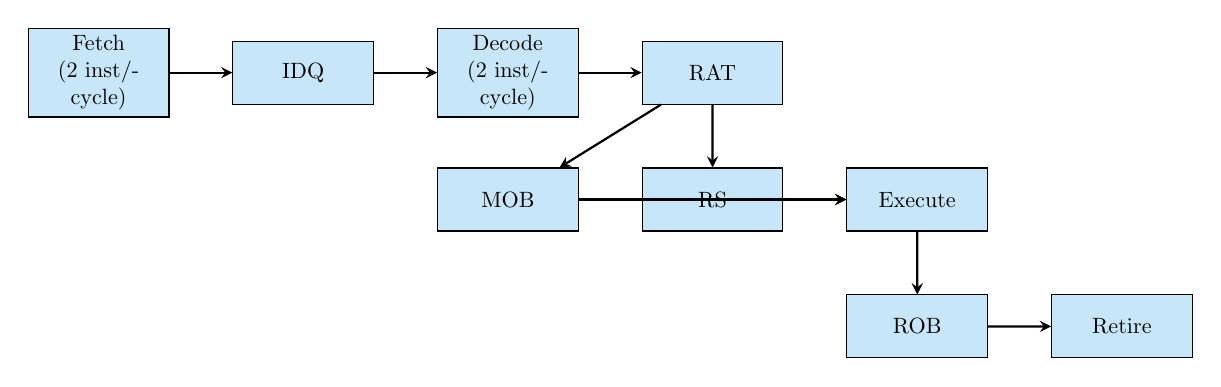
\begin{tikzpicture}[scale=0.8, transform shape]
    % Define styles
    \tikzstyle{block} = [rectangle, draw, fill=lightblue, 
                          text width=2cm, text centered, 
                          minimum height=1cm]
    \tikzstyle{arrow} = [thick,->,>=stealth]
    
    % Create blocks
    \node[block] (fetch) {Fetch\\(2 inst/cycle)};
    \node[block, right=of fetch] (idq) {IDQ};
    \node[block, right=of idq] (decode) {Decode\\(2 inst/cycle)};
    \node[block, right=of decode] (rat) {RAT};
    
    \node[block, below=of rat] (rs) {RS};
    \node[block, right=of rs] (exec) {Execute};
    \node[block, left=of rs] (mob) {MOB};
    
    \node[block, below=of exec] (rob) {ROB};
    \node[block, right=of rob] (retire) {Retire};
    
    % Draw arrows
    \draw[arrow] (fetch) -- (idq);
    \draw[arrow] (idq) -- (decode);
    \draw[arrow] (decode) -- (rat);
    \draw[arrow] (rat) -- (rs);
    \draw[arrow] (rat) -- (mob);
    \draw[arrow] (rs) -- (exec);
    \draw[arrow] (mob) -- (exec);
    \draw[arrow] (exec) -- (rob);
    \draw[arrow] (rob) -- (retire);
\end{tikzpicture}
\end{figure}
\end{frame}

\begin{frame}{Execution Timeline - Second Loop Iteration}
\begin{block}{Question}
Show the system state when completing the fetch of instruction L1 for the second time.
\end{block}

\begin{itemize}
    \item Track instruction flow through pipeline stages
    \item Monitor reservation stations and ROB entries
    \item Identify dependencies and hazards
    \item Calculate execution cycles
\end{itemize}
\end{frame}

\begin{frame}{Key Execution Cycles}
\begin{table}
\centering
\begin{tabular}{|c|l|l|}
\hline
\textbf{Cycle} & \textbf{Operations} & \textbf{Notes} \\
\hline
1 & Fetch first 2 instructions & ADDI R10, SUB R1 \\
\hline
2 & Decode, Fetch next 2 & ADDI R4, LW R5 \\
\hline
3 & Issue to RS/MOB & Load enters MOB \\
\hline
4-6 & Execute ALU ops & Load in progress \\
\hline
7 & Second iteration fetch & RAW dependency \\
\hline
\end{tabular}
\end{table}

\begin{alertblock}{Critical Path}
The load instruction creates a 5-cycle latency that affects dependent instructions.
\end{alertblock}
\end{frame}

\section{Performance Analysis}

\begin{frame}{CPI Calculation}
\begin{block}{Performance Metrics}
\begin{itemize}
    \item Loop contains 10 instructions
    \item Executes 100 iterations
    \item From first LW fetch (cycle 2) to second LW fetch (cycle 7): 5 cycles
    \item No delays from memory reads after first iteration
    \item Structural hazard doesn't cause delays (only 1 instruction in EXE at times)
\end{itemize}
\end{block}

\begin{tcolorbox}[colback=highlightyellow,colframe=darkblue]
\textbf{Result:} CPI $\approx$ 0.5
\begin{itemize}
    \item System can sustain 2 instructions per cycle
    \item OOO execution hides latencies effectively
\end{itemize}
\end{tcolorbox}
\end{frame}

\section{Compiler Optimization}

\begin{frame}[fragile]{Compiler Optimization}
\begin{columns}
\column{0.45\textwidth}
\textbf{Original Code:}
\begin{lstlisting}[basicstyle=\ttfamily\tiny]
R0 = 0
R1 = 0
L1: R4 = 20
    R5 = load 100(R4)
    R3 = R2+2
    R5 = R3 + 2
    R6 = 6
    R7 = R5
    R8 = 8
    R9 = 9
    R1 = R1 + 1
    IF (R1 < 100) goto L1
L2: R4 = 23
\end{lstlisting}

\column{0.45\textwidth}
\textbf{Optimized Code:}
\begin{lstlisting}[basicstyle=\ttfamily\tiny]
R0 = 0
R1 = 0
R4 = 20
R6 = 6
R8 = 8
R9 = 9
L1: R5 = load 100(R4)
    R3 = R2+2
    R5 = R3 + 2
    R1 = R1 + 1
    IF (R1 < 100) goto L1
R7 = R5
L2: R4 = 23
\end{lstlisting}
\end{columns}

\begin{block}{Optimization: Loop Invariant Code Motion}
Move constant assignments outside the loop!
\end{block}
\end{frame}

\begin{frame}{Impact of Optimization}
\begin{block}{Analysis}
\begin{itemize}
    \item \textbf{Before:} 10 instructions in loop
    \item \textbf{After:} 5 instructions in loop
    \item \textbf{BUT:} Load operation still takes 5 cycles
    \item Load operations cannot execute in parallel
\end{itemize}
\end{block}

\begin{alertblock}{Performance Result}
\begin{itemize}
    \item CPI increases by factor of $\approx 2$
    \item IC (Instruction Count) decreases by factor of $\approx 2$
    \item \textbf{Total execution time: No significant change!}
\end{itemize}
\end{alertblock}

\begin{block}{Key Insight}
Runtime = IC × CPI × Clock Period
\end{block}
\end{frame}

\section{Hardware Improvements}

\begin{frame}{Proposed Hardware Enhancement}
\begin{block}{Question}
Adding a third ALU unit - does it improve performance?
\end{block}

\begin{columns}
\column{0.5\textwidth}
\begin{block}{Answer: No}
\begin{itemize}
    \item Structural hazard was not the bottleneck
    \item Load latency dominates execution time
    \item Additional ALU remains unused
\end{itemize}
\end{block}

\column{0.5\textwidth}
\begin{block}{Better Improvements}
\begin{itemize}
    \item Faster load execution (< 5 cycles)
    \item Parallel load execution units
    \item Better memory hierarchy
    \item Prefetching mechanisms
\end{itemize}
\end{block}
\end{columns}
\end{frame}

\section{Conclusions}

\begin{frame}{Key Takeaways}
\begin{enumerate}
    \item \textbf{OOO Execution Benefits:}
    \begin{itemize}
        \item Hides latencies through parallel execution
        \item Achieves CPI < 1 with proper resources
    \end{itemize}
    
    \item \textbf{Memory Operations are Critical:}
    \begin{itemize}
        \item 5-cycle load latency creates bottlenecks
        \item Cannot be easily hidden even with OOO
    \end{itemize}
    
    \item \textbf{Compiler Optimizations:}
    \begin{itemize}
        \item May reduce instruction count
        \item Don't always improve performance
        \item Must consider hardware constraints
    \end{itemize}
    
    \item \textbf{Hardware Improvements:}
    \begin{itemize}
        \item Must target actual bottlenecks
        \item Memory subsystem often more critical than ALUs
    \end{itemize}
\end{enumerate}
\end{frame}

\begin{frame}{Out-of-Order Execution - Cycle 6a}
\scriptsize
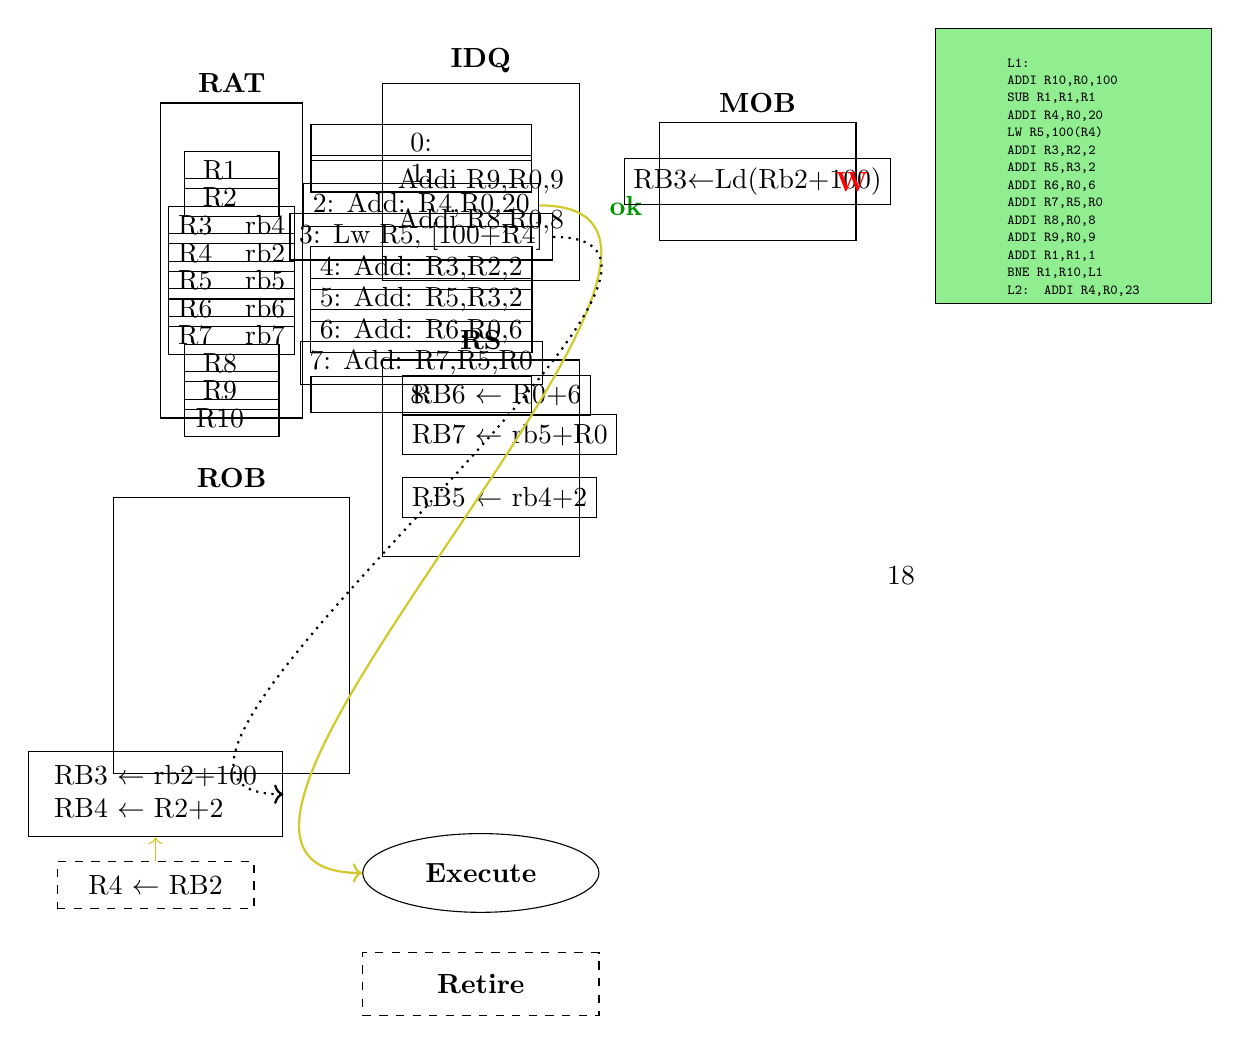
\begin{tikzpicture}[
    box/.style={draw, rectangle, minimum width=1.5cm, minimum height=0.4cm},
    regbox/.style={draw, rectangle, minimum width=1.2cm, minimum height=0.35cm},
    highlightbox/.style={draw, rectangle, minimum width=2.5cm, minimum height=0.35cm, fill=lightgreen},
    roundbox/.style={draw, ellipse, minimum width=3cm, minimum height=1cm},
    dashedbox/.style={draw, dashed, rectangle, minimum width=3cm, minimum height=0.8cm}
]

% RAT (Register Alias Table)
\node[draw, rectangle, minimum width=1.8cm, minimum height=4cm, label=above:{\textbf{RAT}}] (rat) at (0,0) {};
\foreach \i/\val in {1/, 2/, 3/rb4, 4/rb2, 5/rb5, 6/rb6, 7/rb7, 8/, 9/, 10/} {
    \pgfmathsetmacro{\ypos}{1.5 - 0.35*\i}
    \node[regbox] at (0, \ypos) {R\i \hspace{0.3cm} \val};
}

% ROB (Reorder Buffer)
\node[draw, rectangle, minimum width=3cm, minimum height=3.5cm, label=above:{\textbf{ROB}}, below=of rat] (rob) {};
\foreach \i/\inst/\stat in {0//,1//,2/{Add: R4,R0,20}/ok,3/{Lw R5, [100+R4]}/Inv,4/{Add: R3,R2,2}/Inv,5/{Add: R5,R3,2}/Inv,6/{Add: R6,R0,6}/Inv,7/{Add: R7,R5,R0}/Inv,8//} {
    \pgfmathsetmacro{\ypos}{1.5 - 0.4*\i}
    \node[box, minimum width=2.8cm] (rob\i) at ([xshift=1.5cm]rat.east |- 0,\ypos) {\i: \inst};
    \ifnum\i=2
        \node[text=correctgreen] at ([xshift=1.1cm]rob\i.east) {\textbf{ok}};
    \else
        \if\i>2
            \if\i<8
                \node[text=incorrectred] at ([xshift=1.1cm]rob\i.east) {\textbf{Inv}};
            \fi
        \fi
    \fi
}

% IDQ (Instruction Decode Queue)
\node[draw, rectangle, minimum width=2.5cm, minimum height=2.5cm, label=above:{\textbf{IDQ}}, right=of rat, yshift=1cm] (idq) {};
\node at (idq.center) {Addi R9,R0,9};
\node at ([yshift=-0.5cm]idq.center) {Addi R8,R0,8};

% RS (Reservation Station)
\node[draw, rectangle, minimum width=2.5cm, minimum height=2.5cm, label=above:{\textbf{RS}}, below=of idq] (rs) {};
\node[box, anchor=west] at ([xshift=-1cm, yshift=0.8cm]rs.center) {RB6 $\leftarrow$ R0+6};
\node[box, anchor=west] at ([xshift=-1cm, yshift=0.3cm]rs.center) {RB7 $\leftarrow$ rb5+R0};
\node[box, anchor=west] at ([xshift=-1cm, yshift=-0.5cm]rs.center) {RB5 $\leftarrow$ rb4+2};

% MOB (Memory Order Buffer)
\node[draw, rectangle, minimum width=2.5cm, minimum height=1.5cm, label=above:{\textbf{MOB}}, right=1cm of idq] (mob) {};
\node[box] at (mob.center) {RB3$\leftarrow$Ld(Rb2+100)};
\node[text=red] at ([xshift=1.2cm]mob.center) {\textbf{W}};

% Assembly Code Box - using tabular instead of direct text to avoid line break issues
\node[fill=lightgreen, draw, rectangle, minimum width=3.5cm, minimum height=3.5cm, right=1cm of mob, yshift=0.2cm] (code) {
    \begin{tabular}{l}
    \asmcode{L1:}\\
    \asmcode{ADDI R10,R0,100}\\
    \asmcode{SUB R1,R1,R1}\\
    \asmcode{ADDI R4,R0,20}\\
    \asmcode{LW R5,100(R4)}\\
    \asmcode{ADDI R3,R2,2}\\
    \asmcode{ADDI R5,R3,2}\\
    \asmcode{ADDI R6,R0,6}\\
    \asmcode{ADDI R7,R5,R0}\\
    \asmcode{ADDI R8,R0,8}\\
    \asmcode{ADDI R9,R0,9}\\
    \asmcode{ADDI R1,R1,1}\\
    \asmcode{BNE R1,R10,L1}\\
    \asmcode{L2: ADDI R4,R0,23}
    \end{tabular}
};

% Execute and Retire blocks
\node[roundbox, below=3.5cm of rs] (execute) {\textbf{Execute}};
\node[dashedbox, below=0.5cm of execute] (retire) {\textbf{Retire}};

% Bottom boxes showing register mappings
\node[draw, rectangle, minimum width=3cm, minimum height=0.8cm, left=1cm of execute, yshift=1cm] (rb3box) {
    \begin{tabular}{l}
    RB3 $\leftarrow$ rb2+100\\
    RB4 $\leftarrow$ R2+2
    \end{tabular}
};

\node[draw, dashed, rectangle, minimum width=2.5cm, minimum height=0.6cm, below=0.3cm of rb3box] (r4box) {
    R4 $\leftarrow$ RB2
};

% Arrows
\draw[->, thick, yellow!80!black] (rob2.east) to[out=0, in=180] (execute.west);
\draw[->, dotted, thick] (rob3.east) to[out=0, in=180] (rb3box.east);
\draw[->, yellow!80!black] (r4box.north) -- (rb3box.south);

% Page number
\node at (8.5, -4) {18};

\end{tikzpicture}
\end{frame}

% new command for old that has white colorbox
\newcommand{\oldentry}[1]{~#1}
\newcommand{\newentry}[1]{\colorbox{yellow}{#1}}

\begin{frame}{Out-of-Order Execution}
\OOODiagramKV[
]
\end{frame}

\begin{frame}{Out-of-Order Execution: Cycle 1}
\OOODiagramKV[
    % PRF mappings
    idq5=\newentry{SUB~~R1,R1,R1},
    idq6=\newentry{ADDI~R10,R0,100},
 ]
\end{frame}

\begin{frame}{Out-of-Order Execution: Cycle 2}
\OOODiagramKV[
    % PRF mappings
    R1=\newentry{RB1}, R10=\colorbox{yellow}{RB0},
    idq5=\newentry{LW~~~R5,100(R4)},
    idq6=\newentry{ADDI~R4,R0,20},
    rs1=\newentry{RB0$\leftarrow$R0+100},
    rs2=\newentry{RB1$\leftarrow$R1-R1},
    rob11=\newentry{ADDI R10,R0,100},
    rob12=\newentry{INV},
    rob21=\newentry{SUB~~R1,R1,R1},
    rob22=\newentry{INV},
]
\end{frame}

\begin{frame}{Out-of-Order Execution: Cycle 3}
\OOODiagramKV[
    % PRF mappings
    R1=\oldentry{RB1}, R10=\oldentry{RB0},
    R4=\newentry{RB2}, R5=\newentry{RB3},
    idq5=\oldentry{SUB~~R1,R1,R1},
    idq6=\oldentry{ADDI~R10,R0,100},
    rs1=\oldentry{RB0$\leftarrow$R0+100},
    rs2=\oldentry{RB1$\leftarrow$R1-R1},
    rs3=\newentry{RB2$\leftarrow$R0+20},
    rs4=\newentry{RB3$\leftarrow$LD(RB2+100)},
    rob11=\oldentry{ADDI R10,R0,100},
    rob12=\oldentry{INV},
    rob21=\oldentry{SUB~~R1,R1,R1},
    rob22=\oldentry{INV},
    rob31=\newentry{ADDI R4,R0,20},
    rob32=\newentry{INV},
    rob41=\newentry{LW R5,100(R4)},
    rob42=\newentry{INV},
    rs4=\newentry{RB3$\leftarrow$LD(RB2+100)},
    rob42=\newentry{INV},
    mob1=\newentry{RB3$\leftarrow$LD(RB2+100)},
]
\end{frame}

\begin{frame}{Out-of-Order Execution: Cycle 4a}
\OOODiagramKV[
    % PRF mappings
    R1=\oldentry{RB1}, R10=\oldentry{RB0},
    R4=\oldentry{RB2}, R5=\oldentry{RB3},
    idq5=\newentry{ADDI R5,R3,2},
    idq6=\newentry{ADDI R3,R2,2},
    rs3=\oldentry{RB2$\leftarrow$R0+20},
    rs4=\oldentry{RB3$\leftarrow$LD(RB2+100)},
    rob11=\oldentry{ADDI R10,R0,100},
    rob12=\newentry{OK},
    rob21=\oldentry{SUB~~R1,R1,R1},
    rob22=\newentry{OK},
    rob31=\oldentry{ADDI R4,R0,20},
    rob32=\oldentry{INV},
    rob41=\oldentry{LW R5,100(R4)},
    rob42=\oldentry{INV},
    rs4=\oldentry{RB3$\leftarrow$LD(RB2+100)},
    rob42=\oldentry{INV},
    mob1=\oldentry{RB3$\leftarrow$LD(RB2+100)},
]
\end{frame}

\end{document}